\section{Conclusiones y posibles mejoras a aplicar}

\subsection{Mejor modelo para nuestro problema}

Después de realizar todas las pruebas de la sección anterior podemos concluir que el modelo preentrenado en \textbf{ImageNet} que mejor funciona con nuestro dataset es \textbf{EfficientNetB0} tras realizar un Ajuste Fino entrenando previamente la última capa solamente. Este modelo llega a alcanzar un \textbf{0.8627748294162244} de Accuracy. Hay que comentar que si hubiésemos usado una de las últimas versiones de EfficientNet, por ejemplo la B7, posiblemente la Accuracy hubiese sido mejor. No hemos podido hacer la prueba empírica debido al coste computacional que conlleva cargar un modelo con tantos parámetros, pero lo apuntamos como posible mejora.

\subsection{Transferencia de conocimiento de ImageNet}

Tras todas las pruebas y experimentos vemos como el conjunto de nuevas imágenes ha obtenido muy buenos resultados y esto es gracias a los pesos heredados de ImageNet. Como hemos visto en teoría, el conjunto de ImageNet cuenta con mil clases distintas, muchas de ellas ya pertenecientes a comida que aunque no sea en concreto nuestro problema ni sea similar como vimos en la revisión bibliográfica, hemos conseguido alcanzar muy buenos resultados reentrenando estas redes para este problema.

Como conclusión podemos obtener que este paso es muy importante y de gran ayuda en el entrenamiento debido a la gran variedad de clases con las que está entrenado ImageNet, permitiendo que gran cantidad de problemas que podamos encontrar tengan cierta similutud con alguna de las clases de ImageNet.


\subsection{Fallos comunes entre los modelos utilizados}

Al analizar las matrices de confusión nos hemos dado cuenta de que es común para todos los modelos confundir la clase 3 con la clase 7 y viceversa. Tras comprobar el conjunto de datos, podemos ver porque estos se tratan de platos muy similares, por lo que es normal tener un error un poco más alto con estas dos clases. Aun así, se consiguen muy buenos resultados, acertando entre un 80\% de las veces, que aunque es un valor bastante alto, está por debajo del error general.


\begin{figure}[H]
  \centering
  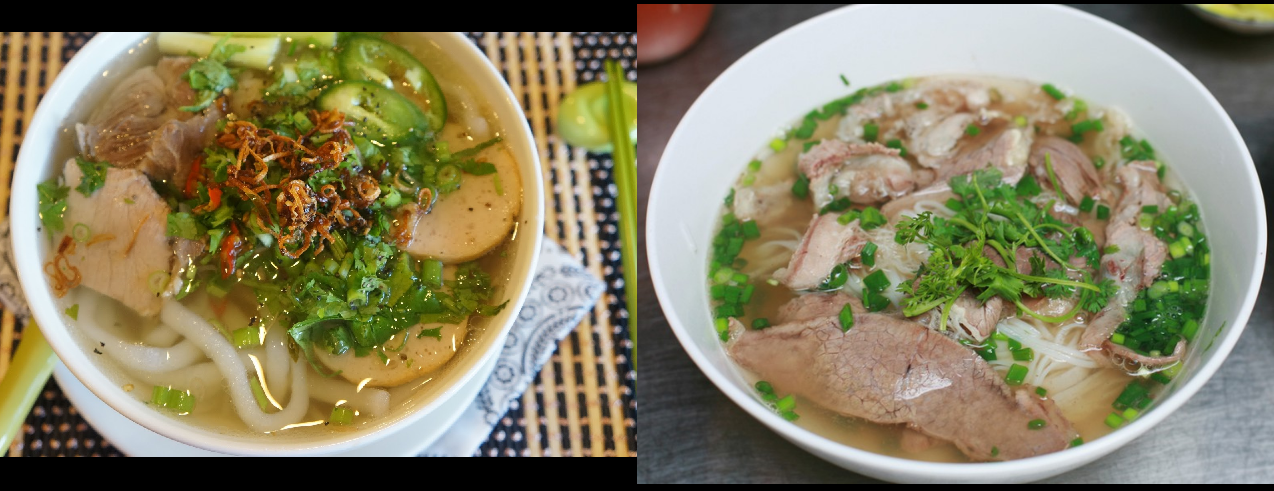
\includegraphics[width=1\linewidth]{Imagenes/cmp-c7-c3.png}
  \caption{Comparación entre dos imágenes de la clase 3 (Banh canh) y 7 (Pho).}
\end{figure}


Como hemos comentado, esto solo es un ejemplo de muchas de las imágenes similares de ambas clases.

\subsection{Posibles soluciones a estos fallos y futuras mejoras}

Los principales problamas comentados podríamos solucionarlos aumentando el conjunto de imágenes de entrenamiento, ya que el principal problema que tiene a la hora de confundir clases es que no tiene suficientes imágenes distintas.

Otro de los problemas que observamos es el sobreajuste. Este problema se presentaba en todas las redes utilizadas en mayor o menor medida, y hemos visto como el añadir al final capas de dropout y batch normalization ha ayudado a evitar este fenomeno, por lo que de cara a resolverlo podríamos probar a introducir más capas de este tipo a lo largo de la red.
